\documentclass[11pt]{article}
\usepackage[margin=2cm]{geometry}
\usepackage{amsmath,amssymb,xcolor,graphicx,booktabs,hyperref}
\graphicspath{{reports/figures/}{figures/}}
\title{Graph Analysis of DiT Token Activations: E-2--E-7}
\author{}
\date{}
\begin{document}
\maketitle
We use 50 trajectories, 450 separate token snapshots, and original 1152-dimensional
features. The fixed illustrative snapshot is golden retriever, replicate 0,
denoiser call 25, block 14. The main detailed graph setting is $k=16$;
large components have at least 32 vertices. All six detailed $k$ settings
have per-component results and plots in the generated-data directory.
\begin{enumerate}
\renewcommand{\labelenumi}{E-\arabic{enumi}}
\setcounter{enumi}{1}
% Requires amsmath, amssymb and xcolor. Paste each blue Answer into its corresponding item.
% Feature dimension 1152; no PCA. All numerical findings are generated from saved results.

% E-2
\item Weighted all-to-all pairwise feature interaction matrix.
{\color{blue}\textbf{Answer:}
For each fixed trajectory, denoiser call, and block, we treat the 256 token observations
as a separate dataset and use their original block-input activations
$f_i=h_i^{\mathrm{in}}\in\mathbb R^{1152}$. We compute the weighted all-to-all interaction
\[
S_{ij}=\exp\!\left(-\frac{\|f_i-f_j\|_2^2}{2\sigma^2}\right),\quad i\ne j,
\qquad S_{ii}=0,
\]
where $\sigma$ is the median positive Euclidean distance over unordered token pairs
in that snapshot. Thus $S$ is symmetric, nonnegative, and has no self-loops.
We construct 450 matrices of size $256\times256$, each with 32,640 unordered
off-diagonal pairs. Computation uses float64 on the saved float16 activations.
All 256 activation rows are distinct within every snapshot, so each observation
maps to one graph vertex without merging duplicate feature vectors.
Updates, positions, and class IDs do not enter the interaction calculation.
The bandwidth is held fixed when changing $k$. This is an activation-distance
affinity, not a model attention-weight matrix. Because the bandwidth is the
median distance, the median affinity is approximately $\exp(-1/2)$ by construction;
this should not be interpreted as an empirical structural discovery.
}


% E-3
\item kNN graph construction and connected components.
{\color{blue}\textbf{Answer:}
For each token $i$, we select the $k$ largest off-diagonal affinities,
equivalently the $k$ smallest Euclidean distances. Exact ties are resolved by
token index. Let $B_{ij}^{(k)}$ indicate that $j$ is selected by $i$. We use
\[
A_{ij}^{(k)}=\mathbf{1}\{B_{ij}^{(k)}=1\ \mathrm{or}\ B_{ji}^{(k)}=1\},
\qquad W_{ij}^{(k)}=S_{ij}A_{ij}^{(k)}.
\]
This union symmetrization gives an undirected, weighted kNN graph. Connected
components are computed on its unweighted support. We scan every integer
$k=2,\ldots,64$, producing 28,350 graph records. Of 450 snapshots,
315 are connected at $k=2$, and all are connected by $k=15$.
Here $k_c$ is the smallest connected value within the scanned range; graphs may
already be connected at $k=1$. Component counts are nonincreasing because the
edge sets are nested. At $k=2$, the mean component counts are 3.08 for call 25/block 24
and 3.88 for call 40/block 24. The fixed representative snapshot is connected
throughout the scanned range.
}


% E-4
\item Combinatorial connectivity analysis.
{\color{blue}\textbf{Answer:}
We predefine a large component as one with at least 32 vertices.
Detailed component analysis is performed at $k=2,4,8,16,32,64$, with $k=16$
as the main setting. Every main-setting graph has one 256-vertex component.
For each component, the unweighted degree is $d_i^{(0)}=\sum_j A_{ij}$ and
the local clustering coefficient is
$C_i=2T_i/[d_i^{(0)}(d_i^{(0)}-1)]$, where $T_i$ counts triangles incident
to $i$. We plot both empirical distributions for all 2739 large-component cases.
Union symmetrization permits degrees larger than $k$.
For the representative at $k=16$, degrees range from 16
to 61, with mean 22.508
and skewness 2.095; the distribution is right-skewed.
Its clustering coefficients range from 0.178
to 0.617, with mean
0.359 and mild positive skewness
0.545.
Across the 450 main graphs, all degree distributions have sample skewness above 0.5;
315 clustering distributions have absolute skewness at most 0.5 and 135 have
positive skewness above 0.5. These are empirical shape descriptions;
we do not claim a fitted normal, Poisson, or power-law family.
}


% E-5
\item Laplacian spectral analysis and nodal domains.
{\color{blue}\textbf{Answer:}
For each large component, we use the retained Gaussian weights and form
\[
D=\operatorname{diag}(W\mathbf{1}),\qquad
\widehat L=I-D^{-1/2}WD^{-1/2}.
\]
We record $\lambda_2(k)$ whenever the whole snapshot graph is connected and
plot the 32 smallest eigenvalues for every detailed component. In 51/450
curves, $\lambda_2(k)$ has at least one decrease, so normalized-Laplacian
connectivity is not assumed monotone with $k$.
The baseline three-dimensional invariant subspace is spanned by $q_2,q_3,q_4$.
To choose a nodal eigenvector, we search indices $j=2,\ldots,\min(32,|G|-1)$ for a positive
eigenvalue with both adjacent gaps at least $10^{-6}$ and
$\min(\lambda_j-\lambda_{j-1},\lambda_{j+1}-\lambda_j)/\lambda_j\ge0.05$.
Among qualifying candidates, we maximize the minimum adjacent gap. The next
eigenvalue beyond the displayed spectrum is also checked when necessary.
For the representative, $\lambda_2=0.071018$ and
the selected eigenpair is $\lambda_3=0.225608$,
with adjacent gaps 0.154591 and
0.102824.
Its $q_3$ produces 2 strict nodal domains.
Each domain is a connected component of the positive or negative induced
subgraph, rather than simply all vertices with the same sign. Numerical zeros
are marked separately using tolerance $10^{-10}\|q_j\|_\infty$.
We color the vertices in the embedding spanned by $q_3,q_2,q_4$ and on the
16-by-16 token grid.

At $k=16$, 17/450 graphs have no qualifying eigenvalue; across all detailed
components, 125/2739 lack one. These cases are explicitly reported
without manufacturing a nodal partition.
The representative domains contain 131 and 125 tokens,
with mean update norms 143.73 and
159.76. Their within-domain standard deviations
are 44.52 and 54.71;
the partition explains only 2.53\%
of update-norm variance. The spatial overlay shows broad organization and
does not accurately trace the object boundary. It is a nominal latent-token
grid correspondence, not pixel-level semantic ground truth.
}


% E-6
\item Optional clustering comparison.
{\color{blue}\textbf{Answer:}
As an optional baseline, we apply two-cluster k-means directly to the
original activation vectors, using five fixed-seed k-means++ initializations
and 50 iterations per initialization, then retain the lowest-inertia solution.
The graph remains unchanged. For the representative, the k-means partition
has normalized cut 0.204739.
For the selected two-domain nodal partition, normalized cut is
0.362188 and the adjusted Rand index
between the two partitions is 0.0119.
These compare unsupervised partitions; they do not measure semantic accuracy.
Objective/partition comparisons are reported only where a full two-domain
nodal partition is available, to keep the number of groups comparable.
This applies to 348/450 snapshots, spanning
50 trajectories. Averaging the available comparable
snapshots within each trajectory, then across trajectories, gives a mean
partition ARI of 0.358. This summary is conditional on
the availability of a two-domain nodal partition. The chosen nodal eigenvector
uses the separation rule, rather than minimizing normalized cut.
}


% E-7
\item Preliminary findings.
{\color{blue}\textbf{Answer:}
The graph structure varies with depth and denoising stage. At $k=16$,
mean clustering rises from 0.303 at call 10/block 4 to 0.503 at call 40/block 24.
The corresponding mean Fiedler values are 0.373 and 0.053. Together with
greater fragmentation at small $k$, this suggests stronger local organization
and weaker global connectivity in several later/deeper settings, although
the trend is not universal.

We also treat recorded updates as graph signals. For scalar $u_i=\|r_i\|_2$
and vector $r_i$, graph energy is $\sum_{i<j}W_{ij}\|z_i-z_j\|^2$.
We compare it with the exact expectation under uniformly permuting node values
on the same graph:
\[
\mathbb E_{\pi} E(z_{\pi})=
\frac{2\sum_{i<j} W_{ij}}{n-1}
\sum_i\|z_i-\bar z\|^2.
\]
At $k=16$, mean observed-to-null ratios are
0.629 for update magnitude,
0.617 for the full update vector, and
0.694 for spatial coordinates.
Edge-weighted update cosine is 0.676,
compared with 0.510 over all unordered pairs.
Thus activation-neighbor relationships are associated with update and spatial
organization. These averages first summarize the nine snapshots within each
trajectory, then average over 50 trajectories; they do not treat tokens as
independent replicates.

Mean top-16 neighbor retention across layers is
0.505 for $4\to14$,
0.539 for $14\to24$, and
0.288 for $4\to24$, versus $16/255\approx0.063$
for independent uniform neighbor sets. This motivates later investigation
of cross-layer graph transfer. Spatial coherence may explain part of these
associations. We have not measured correction accuracy, rollout quality,
or inference speed, so these findings do not establish correction or reuse
performance. All results are conditional on this checkpoint, sampler,
ten fixed classes, and saved activation precision.
}

\end{enumerate}
\clearpage
\begin{figure}[p]
\centering
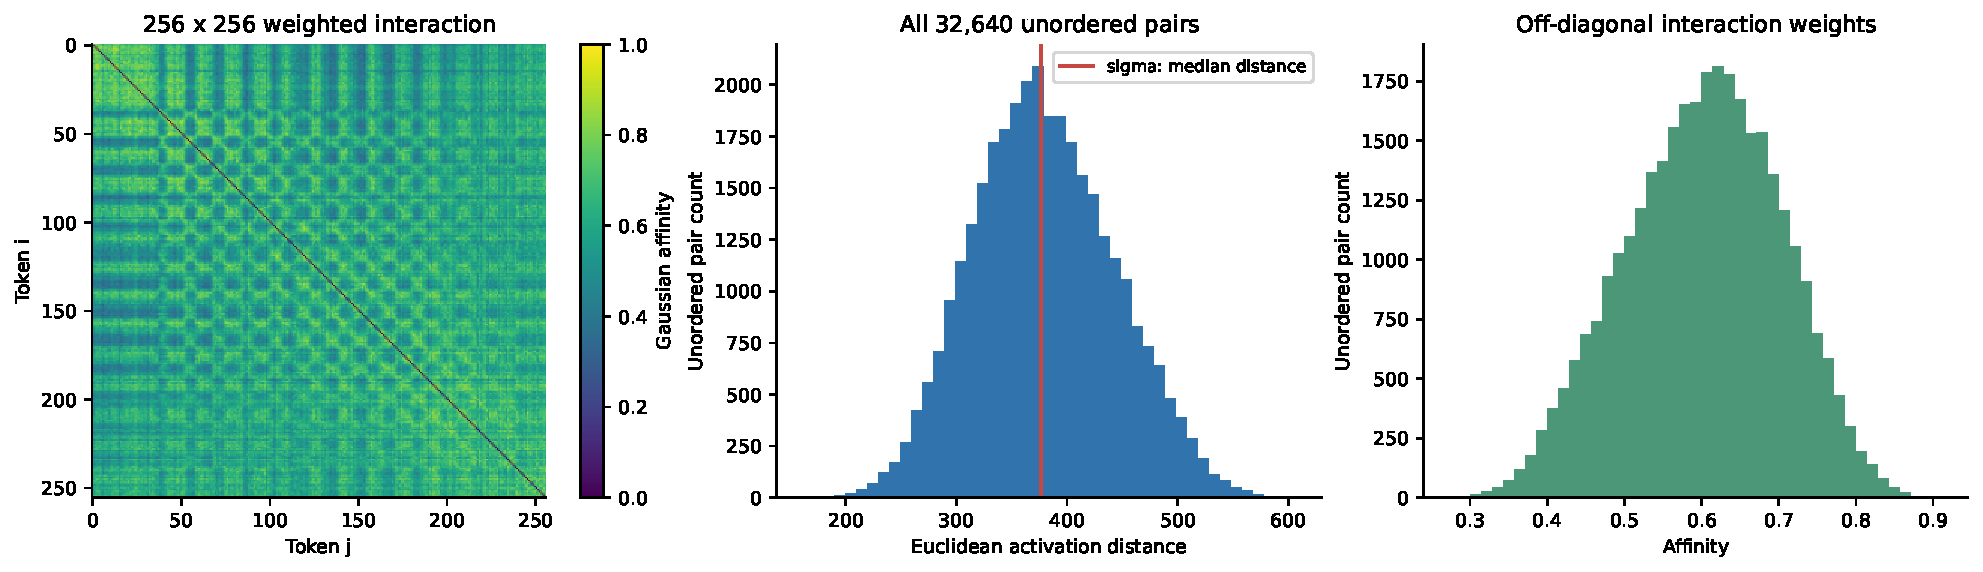
\includegraphics[width=\linewidth]{e2_pairwise_interactions.pdf}
\caption{E-2: weighted interaction matrix and pair distributions.}
\end{figure}
\begin{figure}[p]
\centering
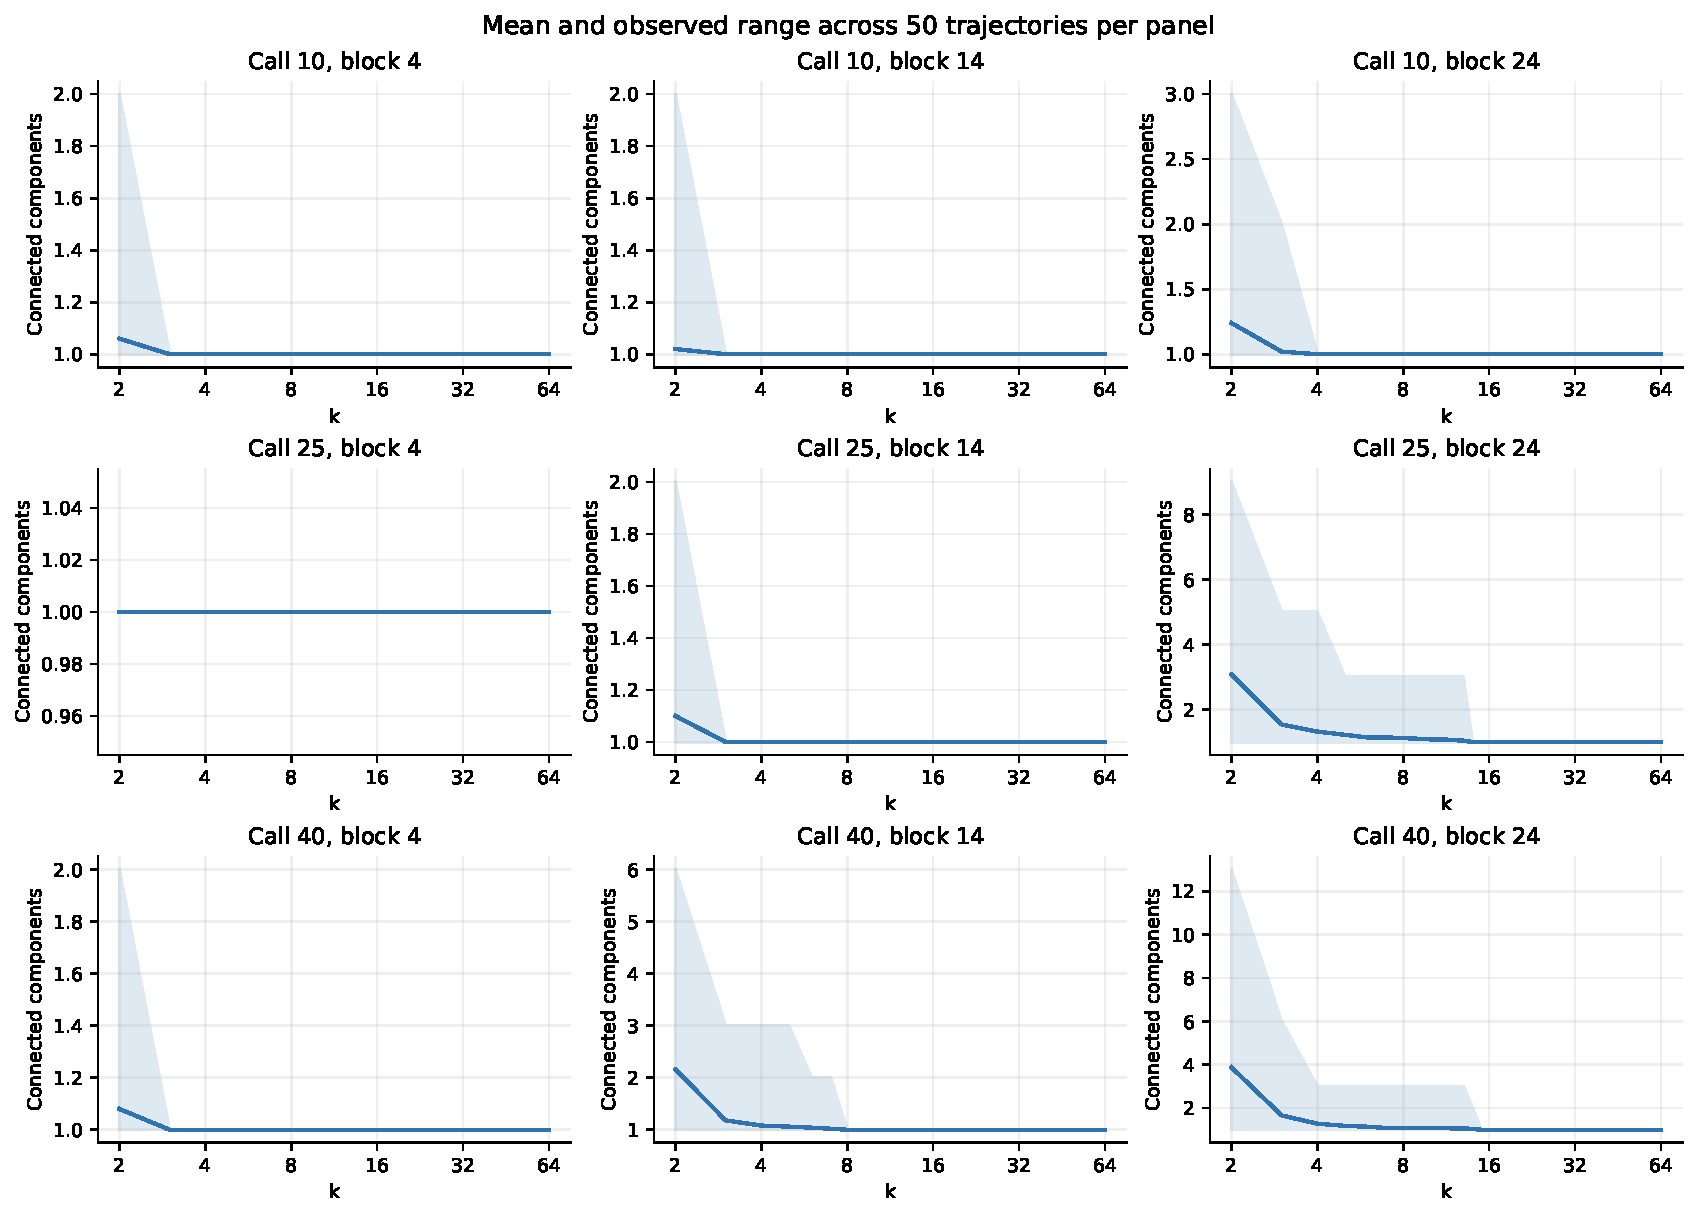
\includegraphics[width=\linewidth]{e3_connectivity_all.pdf}
\caption{E-3: component-count curves; mean and observed range over 50 trajectories per condition.}
\end{figure}
\begin{figure}[p]
\centering
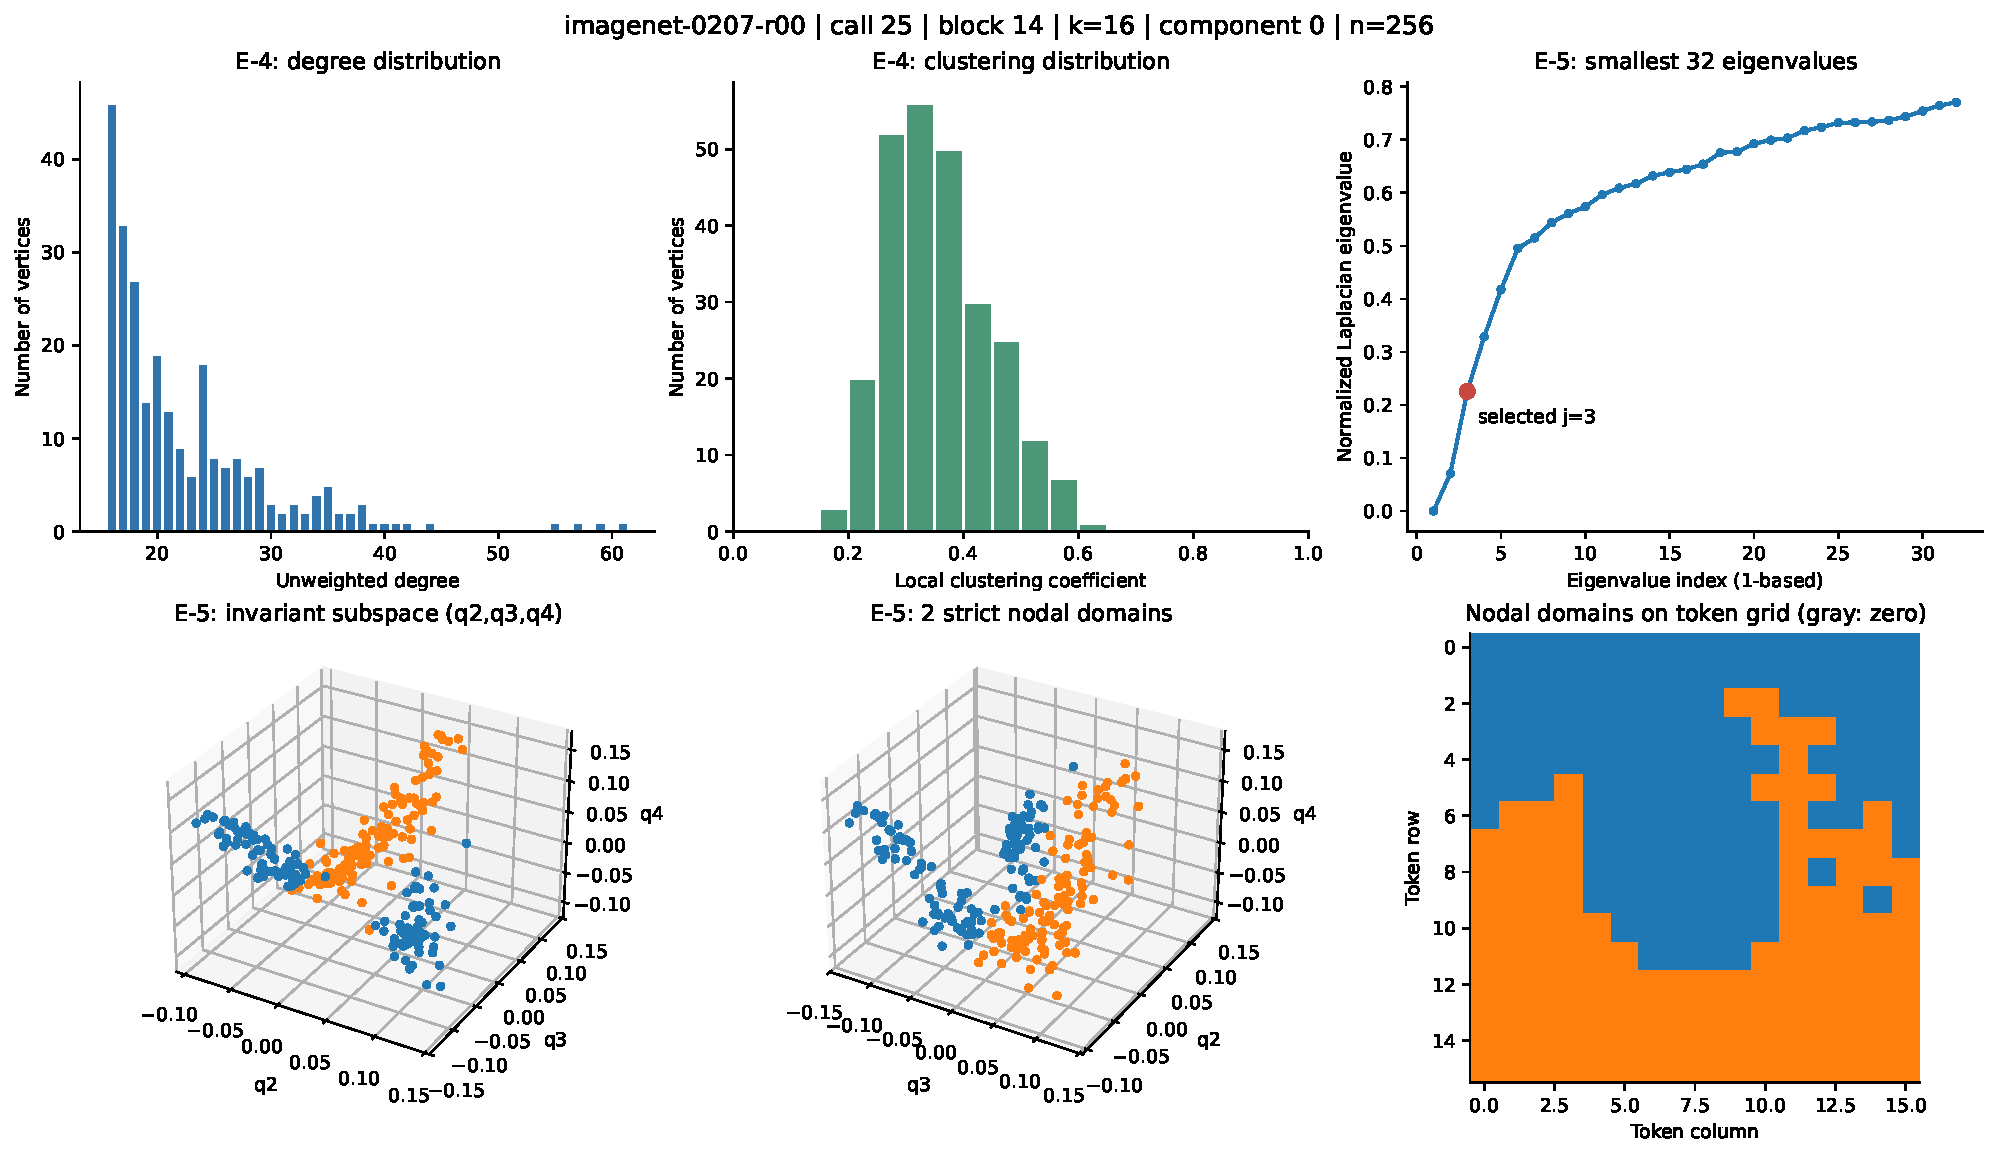
\includegraphics[width=\linewidth]{e4_e5_k16_component00.pdf}
\caption{E-4/E-5: representative degree, clustering, spectrum, embeddings and nodal domains.}
\end{figure}
\begin{figure}[p]
\centering
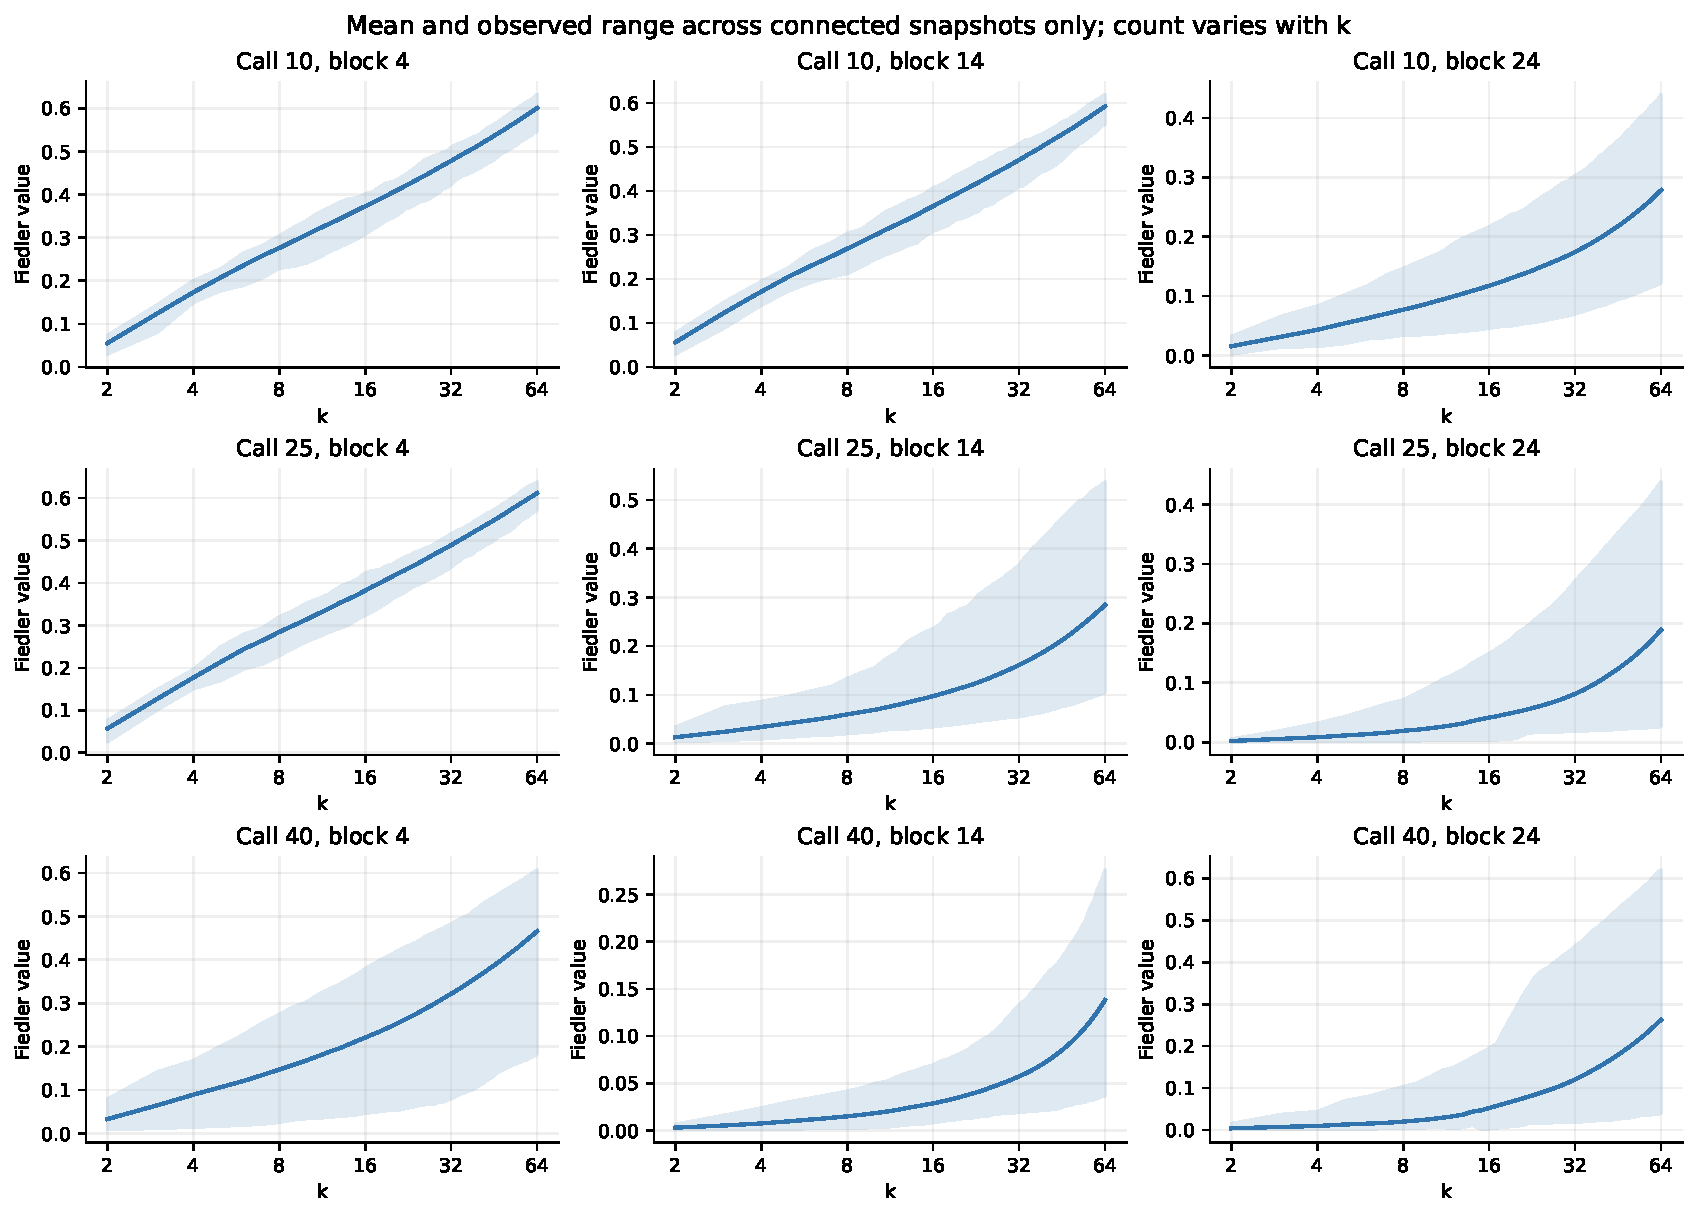
\includegraphics[width=\linewidth]{e5_fiedler_all.pdf}
\caption{E-5: mean and observed range of Fiedler values among connected graphs.}
\end{figure}
\begin{figure}[p]
\centering
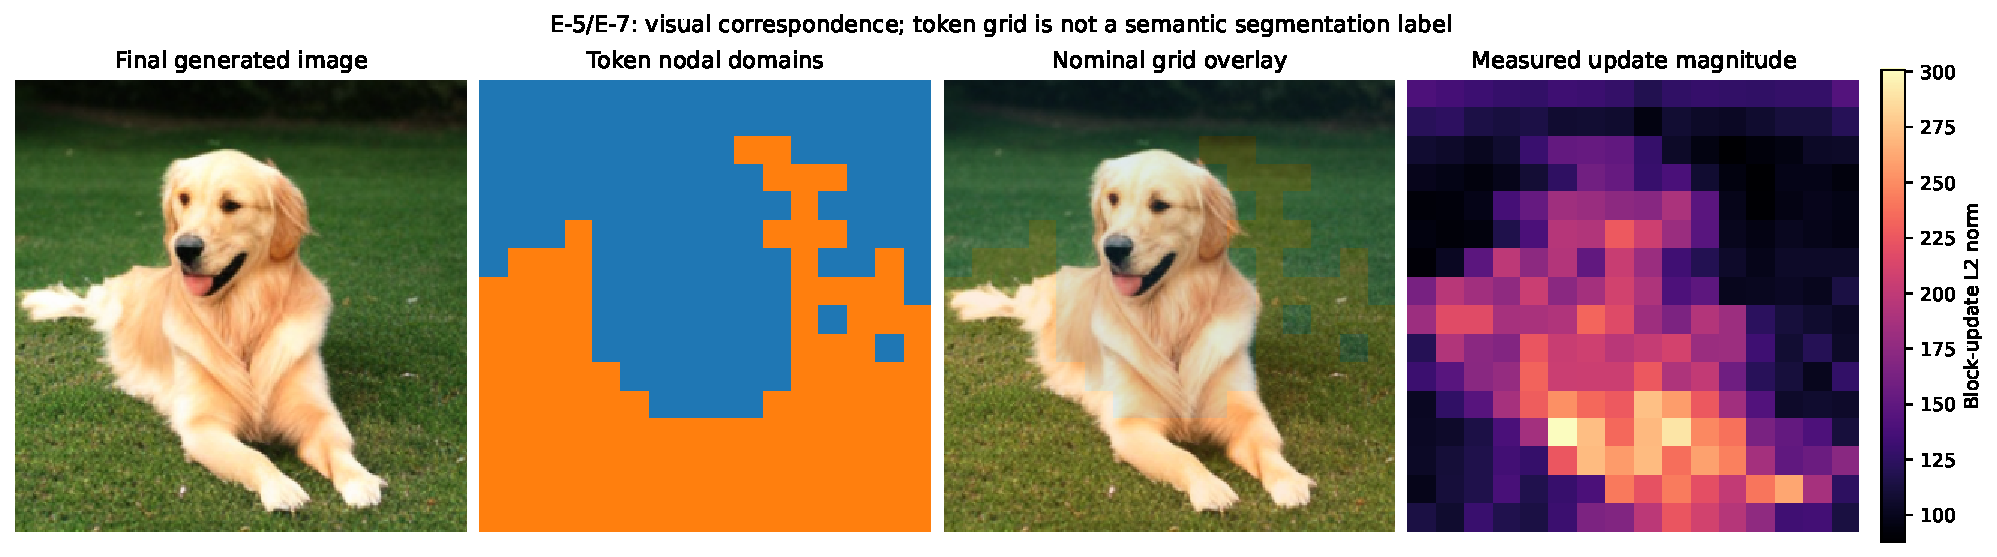
\includegraphics[width=\linewidth]{e5_e7_original_data.pdf}
\caption{E-5/E-7: nodal domains, final image and measured updates.}
\end{figure}
\begin{figure}[p]
\centering
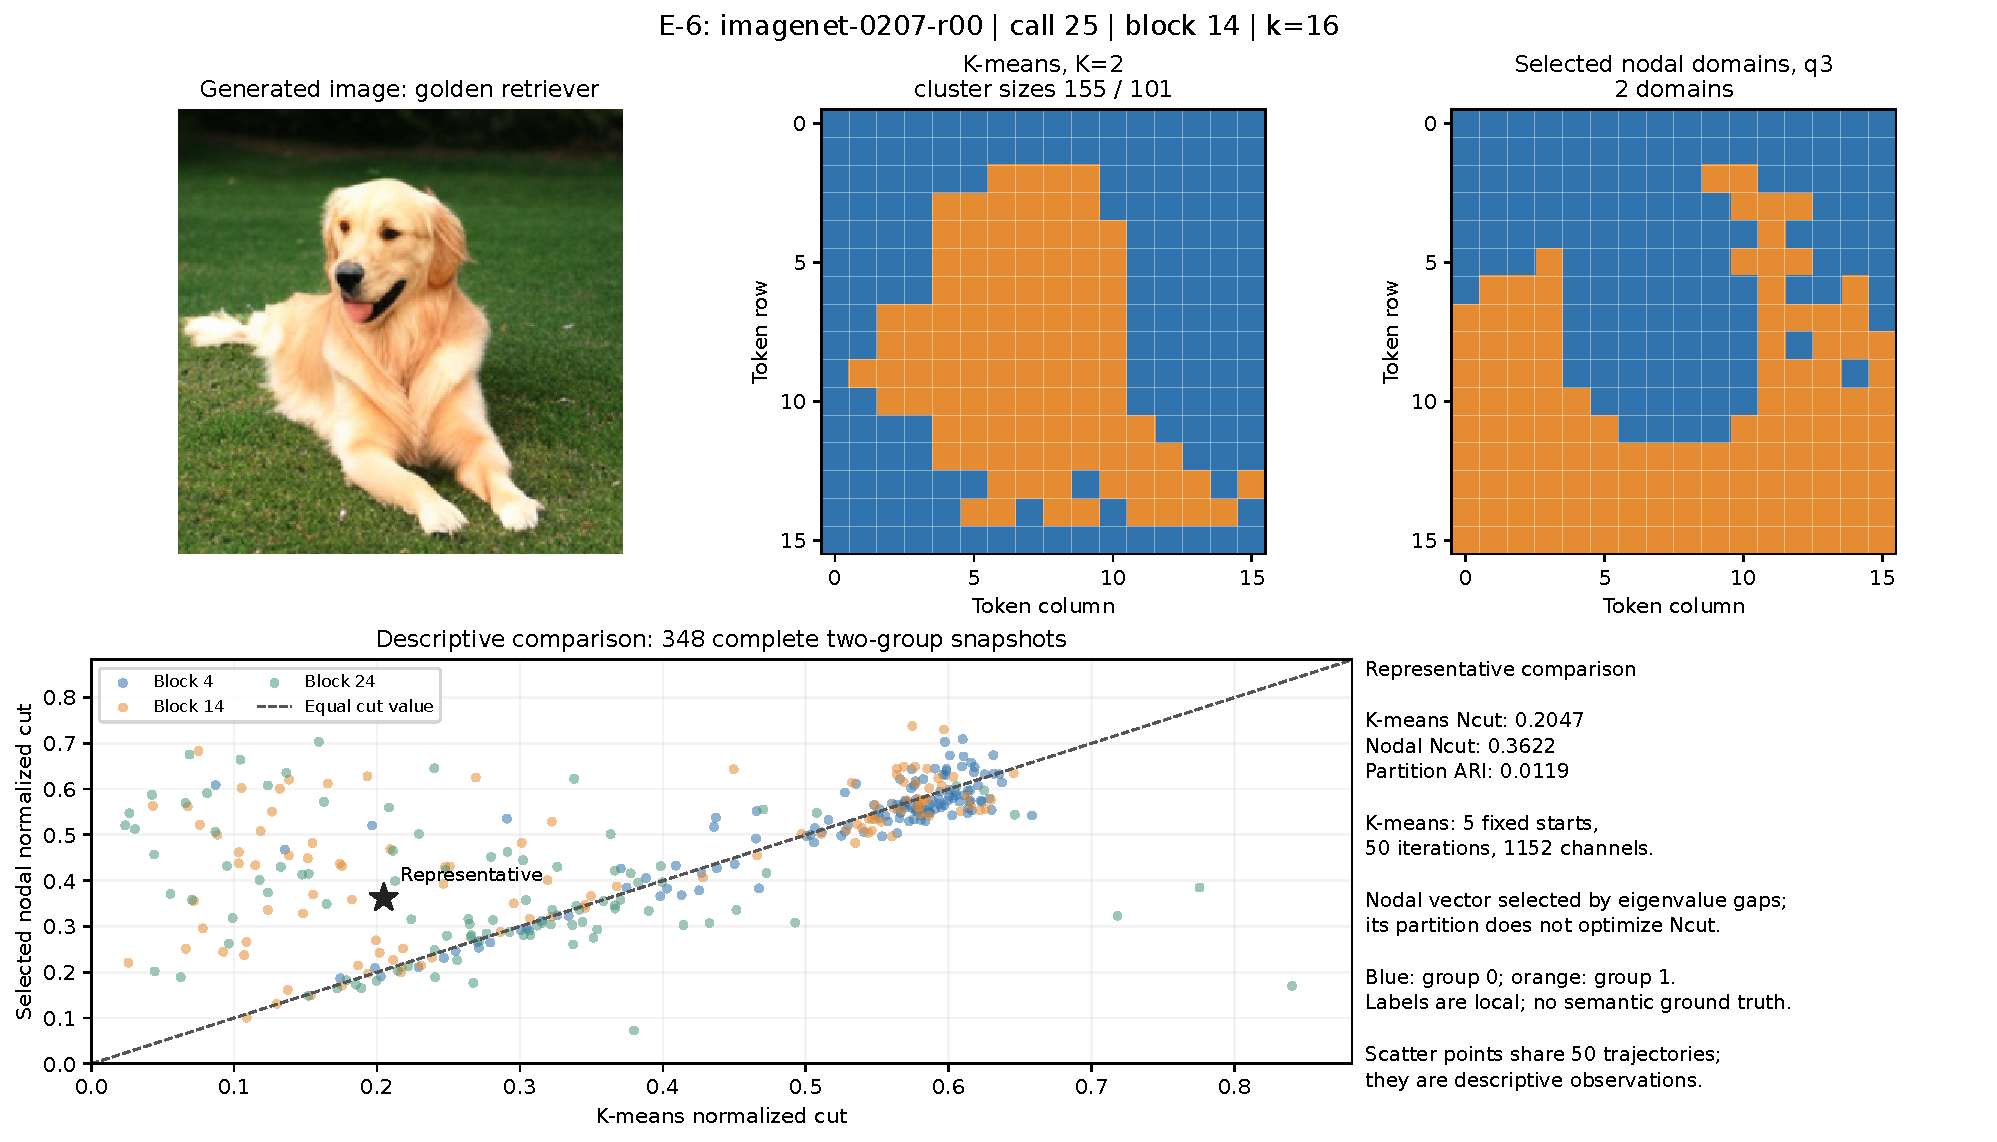
\includegraphics[width=\linewidth]{e6_clustering_comparison.pdf}
\caption{E-6: two-cluster k-means and selected nodal partitions; comparisons conditional on two complete domains.}
\end{figure}
\begin{figure}[p]
\centering
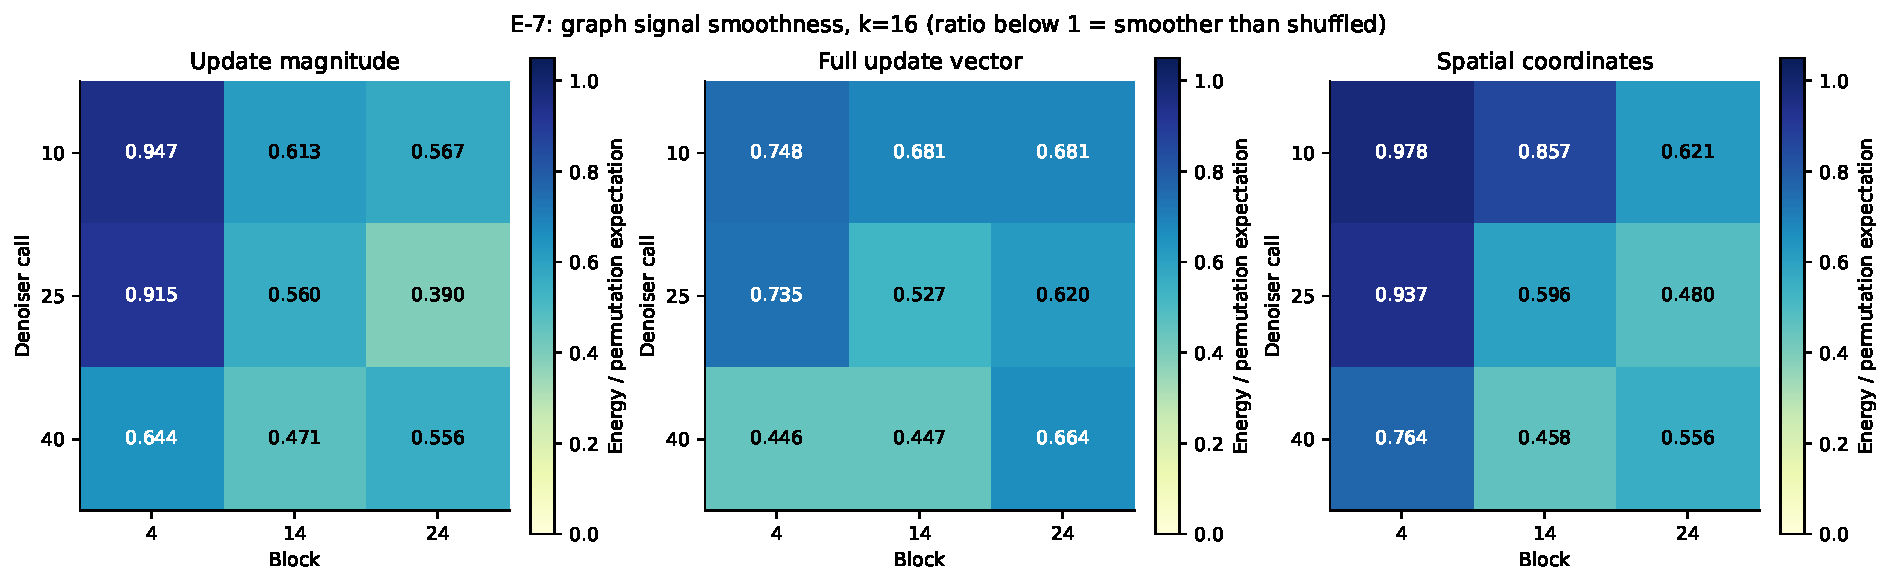
\includegraphics[width=\linewidth]{e7_attribute_smoothness.pdf}
\caption{E-7: graph-signal energy relative to random node permutations.}
\end{figure}
\begin{figure}[p]
\centering
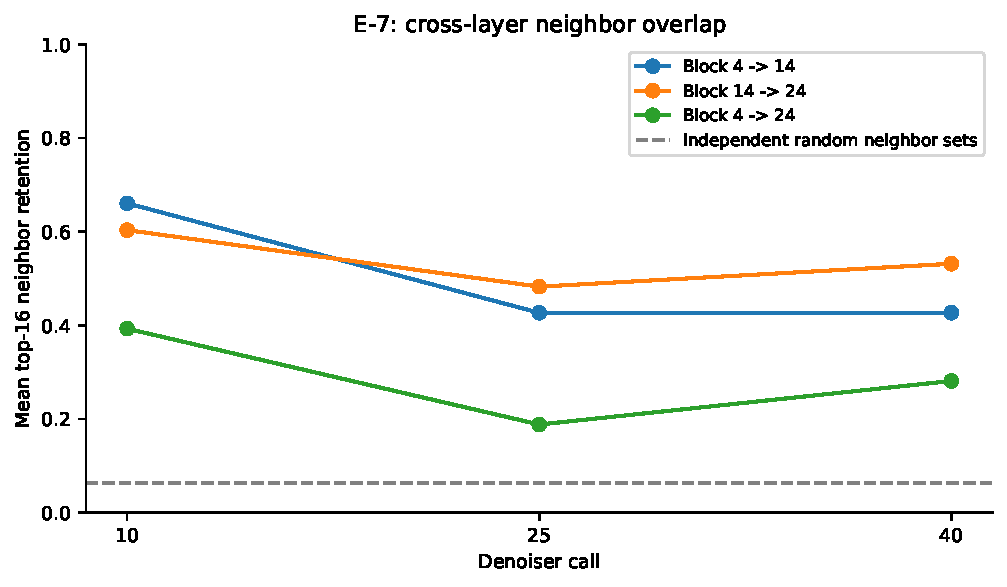
\includegraphics[width=\linewidth]{e7_cross_layer_neighbors.pdf}
\caption{E-7: same-token neighbor retention across layers.}
\end{figure}
\clearpage
\begin{thebibliography}{9}
\bibitem{luxburg} U. von Luxburg, A Tutorial on Spectral Clustering, 2007.
\url{https://www.cs.columbia.edu/~jebara/6772/papers/Luxburg07_tutorial.pdf}
\bibitem{nodal} E. B. Davies, G. M. L. Gladwell, J. Leydold and P. F. Stadler,
Discrete Nodal Domain Theorems, 2001.
\end{thebibliography}
\end{document}
